\chapter{Un semplice documento \LaTeX}

Riportiamo di seguito il codice sorgente di un breve documento
\LaTeX, che pu\`o costituire un esempio utile
per redigere la relazione di un'esperienza didattica.
Il codice \`e volutamente non commentato, in modo da non risultare
troppo appesantito; le informazioni contenute nel capitolo
\ref{chap:LaTeX} dovrebbero essere pi\`u che sufficienti per
ricostruire il significato dei singoli comandi.
Il risultato della compilazione \`e riportato di seguito,
in figura \ref{fig:TemplateLaTeX}.

\begin{verbatim}
\documentclass[a4paper, 10pt]{article}
\usepackage[dvips]{graphicx}
\usepackage[italian]{babel}

\begin{document}
\title{\LaTeX: un \emph{template} per le relazioni}
\author{L. Baldini - INFN Pisa}
\maketitle

\section{La nostra prima sezione}
In questa sezione parliamo di equazioni. Ma prima notiamo che in
\LaTeX\ si pu\`o andare a capo con un \verb|\\|\\
oppure lasciando una linea vuota, nel qual caso la linea
successiva \`e indentata.

\subsection{Equazioni}
Ma veniamo dunque alle equazioni\ldots
\begin{equation}
\int_{-\infty}^{\infty} e^{-x^2} dx = \sqrt{\pi}
\end{equation}

\section{Tabelle, elenchi e figure}

La tabella \ref{UnaTabella} \`e il nostro primo esempio di tabella,
mentre la figura \ref{UnaFigura} \`e, appunto, una figura.

\begin{table}[htb!]
\begin{center}
\begin{tabular}{cc}
\hline
Colonna 1 & Colonna 2\\
\hline
\hline
a & b \\
c & d \\
\hline
\end{tabular}
\caption{Un esempio di tabella\ldots}
\label{UnaTabella}
\end{center}
\end{table}

\noindent In \LaTeX\ \`e facile fare elenchi:
\begin{enumerate}
\item{Punto primo.}
\item{Punto secondo.}
\end{enumerate}

\begin{figure}[htb!]
\begin{center}
\includegraphics[height=3cm, angle=270]{figura.eps}
\caption{Questa \`e una figura. Piccola, lo ammetto, ma pur sempre
una figura.}
\label{UnaFigura}
\end{center}
\end{figure}

\end{document}
\end{verbatim}

\panelfig
{\framebox{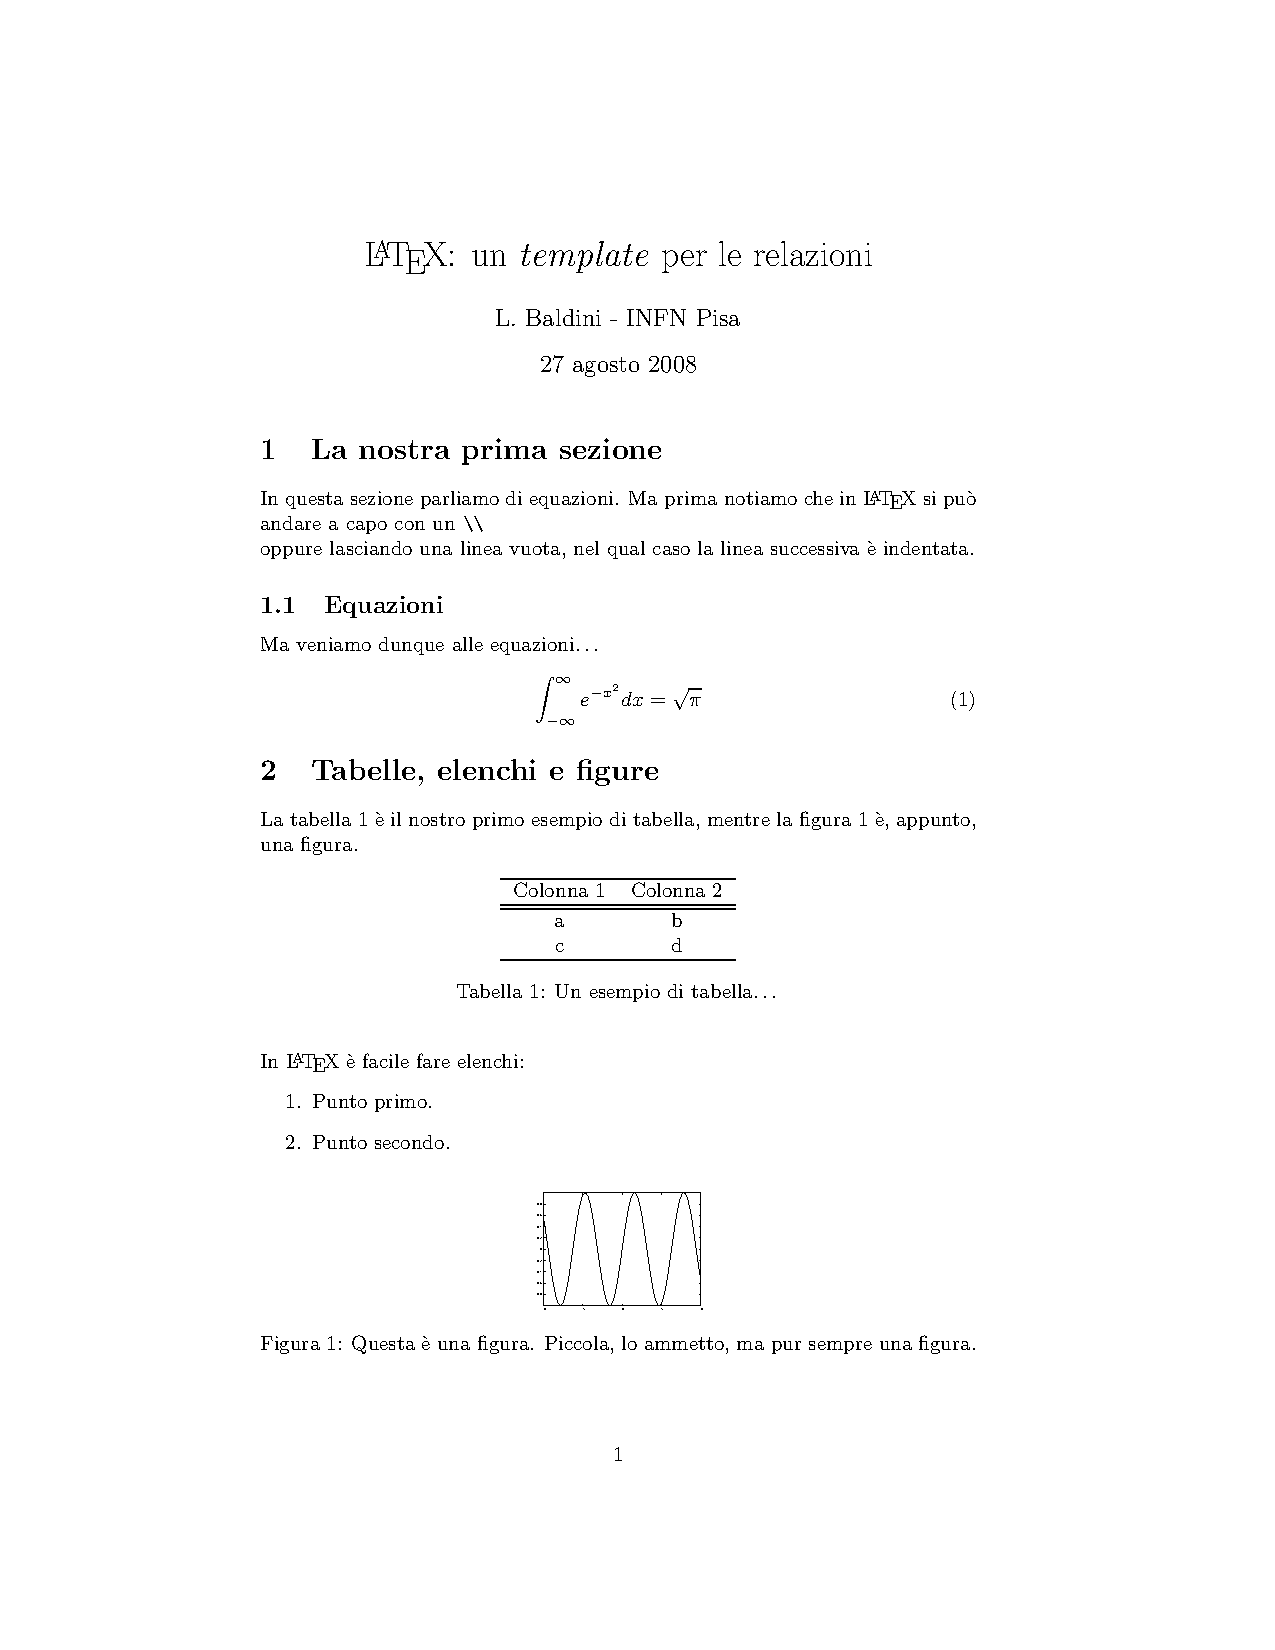
\includegraphics[width=\textwidth]{./aa_LaTeX/figure/template.pdf}}}
{Risultato della compilazione del documento \LaTeX\ di esempio.}
{fig:TemplateLaTeX}

